\section{Mode d'emploi}

Pour lancer le serveur et les clients, nous avons réalisé deux scripts shell. Le fichier \verb|server.sh| ressemble à un démon qui empêche le lancement en double du server et permet de le controler en utilisant les commandes start, stop et restart... De son côté, le fichier client.sh permet de lancer un xterm par client afin d'agir sur ceux-ci.

Evidemment, il est possible de lancer le tout à la main. Auquel cas la syntaxe de lancement du client est la suivante : \verb|client/client <Nom du client> <port>|. Le serveur quand à lui n'attend pas de paramètres sur la ligne de commande et se lance par : \verb|server/server|.

Pour compiler le tp tapez simplement make dans le dossier client pour le client, et dans le dossier server pour le server. La doc pour chaque projet a été générée pour doxygen et est disponible via \verb|doc/html/index.html| dans le dossier client pour le client, et dans le dossier server pour le server.

\section{Problèmes rencontrés et solutions}
\subsection{Terminaison du serveur}

La gestion simplifié des RPC que nous avons utilisée (usage des fonctions registerrpc et callrpc) empêchent la terminaison du serveur une fois les trois clients connectés. Il serait évidemment possible pour ceux-ci de signaler qu'ils exécutent l'algorithme de Ricart et Agrawala au serveur pour que celui-ci se termine (à l'aide d'une nouvelle fonction RPC \verb|we_are_all_set| par exemple). Mais une telle méthodologie ne nous plaisait pas.

c'est pour cette raison que nous avons choisi de gérer proprement la terminaison du programme sur un \verb|Ctrl+C|, correspondant au signal 2 (\verb|SIG_INT|) et écrit un démon permettant de quitter et de relancer le serveur à volonté. La vraie solution, selon nous, serait d'utiliser les méthodes avancées de programmation des RPC (via les fonctions \verb|svc_*|) beaucoup plus polyvalentes.

Lorsque l'on exécute un \verb|Ctrl+C| pour fermer le serveur, celui-ci se détache du portmaper. Il a suffit d'armer le signal 2 au lancement de l'application, pour pouvoir le catcher au moment opportun, libérer les ressources utilisées, et fermer le serveur.

\subsection{Le multiplexage des I/O grace à ``select''}

L'écriture de ce programme a été l'occasion de découvrir la fonction \verb|select| définie dans le fichier \verb|unistd.h|. Celle-ci permet de mettre le programme en attente sur deux descripteurs de fichiers (à la fois l'entrée standard et la socket). Sans cette fonction \verb|select|, nous aurions été réduits à gérer deux threads avec tous les problèmes de partage de ressources que cela implique.

\subsection{Ce n'est pas de l'objet}

De manière un peu moins technique (et un peu plus philosophique...), nous avons éprouvé quelques difficultés à revenir au C après avoir fait du Java ou du C++ voir du Python durant nos stages et projets à l'ISIMA. Néanmoins, ce retour aux sources nous a permis d'apprécier une nouvelle fois la toute puissance de Vim (complétion du code, syntaxe, gestion des fenêtres, des onglets, auto-indentation) et d'exploiter pleinement le potentiel de git (système de gestion de version distribué).

\section{Un Cas d'utilisation}

La section qui suit présente les communications mises en jeu lors du cas simple où les clients demandent tour à tour leur entrée en section critique, du premier au dernier. Voici tout d'abord la trace fournie par chaque client, puis le graphique correspondant. La correspondance entre les deux prouve que les horloges sont correctement gérées.

\paragraph{Client 1 : \\}

        \begin{minipage}{0.90\textwidth}
                \begin{lstlisting}
+++ Broadcasted message : Req(1, 1)
--- Received message : Req(1, 1)
--- Received message : Ack(3, 2)
--- Received message : Ack(3, 3)
Entering critical section.
..........
Leaving critical section.
--- Received message : Req(4, 2)
+++ Sent message : Ack(7, 1)
--- Received message : Req(7, 3)
+++ Sent message : Ack(9, 1)
                \end{lstlisting}
        \end{minipage}


\paragraph{Client 2 :\\}

        \begin{minipage}{0.90\textwidth}
                \begin{lstlisting}

--- Received message : Req(1, 1)
+++ Sent message : Ack(3, 2)
e
+++ Broadcasted message : Req(4, 2)
--- Received message : Req(4, 2)
--- Received message : Ack(6, 3)
--- Received message : Req(7, 3)
--- Stacking Ack message for client 3
--- Received message : Ack(7, 1)
Entering critical section.
..........
Leaving critical section.
+++ Sent message : Ack(10, 2)
\end{lstlisting}
        \end{minipage}

\paragraph{Client 3 :\\ }

        \begin{minipage}{0.90\textwidth}
                \begin{lstlisting}
--- Received message : Req(1, 1)
+++ Sent message : Ack(3, 3)
--- Received message : Req(4, 2)
+++ Sent message : Ack(6, 3)
e
+++ Broadcasted message : Req(7, 3)
--- Received message : Req(7, 3)
--- Received message : Ack(9, 1)
--- Received message : Ack(10, 2)
Entering critical section.
..........
Leaving critical section.

\end{lstlisting}
        \end{minipage}
\begin{center}
\begin{figure}[H]
	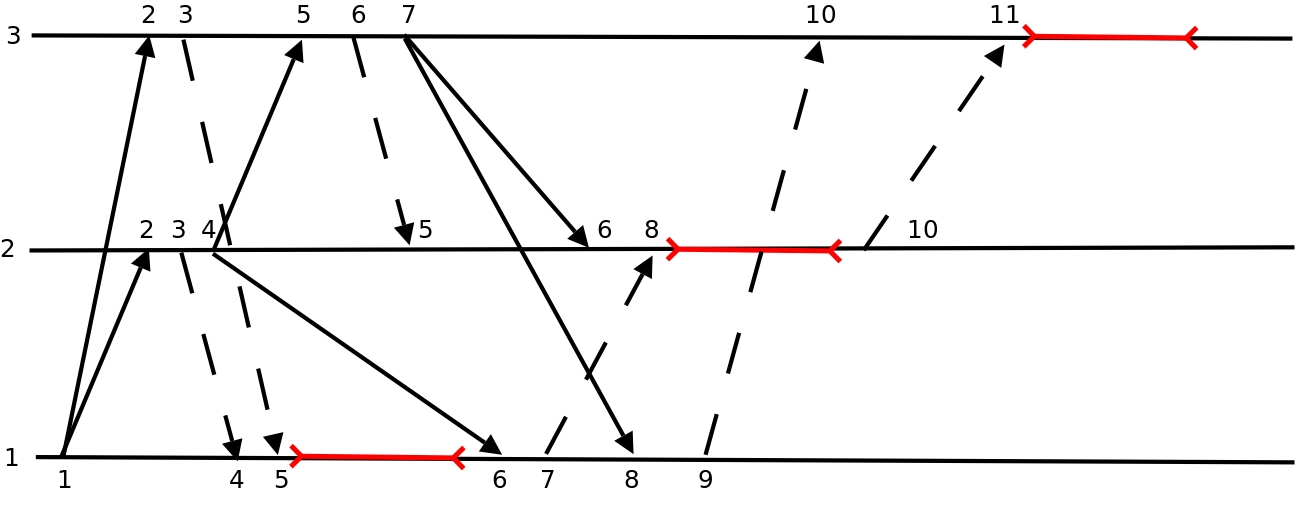
\includegraphics[width=\textwidth]{images/casUtil.png}
\caption{CallFlow de l'éxecution du cas d'utilisation}
\end{figure}
\end{center}